\documentclass[14pt]{beamer}
\usepackage{./Estilos/BeamerUVM}
\usepackage{./Estilos/ColoresLatex}
\usetheme{Madrid}
\usecolortheme{default}
%\useoutertheme{default}
\setbeamercovered{invisible}
% or whatever (possibly just delete it)
\setbeamertemplate{section in toc}[sections numbered]
\setbeamertemplate{subsection in toc}[subsections numbered]
\setbeamertemplate{subsection in toc}{\leavevmode\leftskip=3.2em\rlap{\hskip-2em\inserttocsectionnumber.\inserttocsubsectionnumber}\inserttocsubsection\par}
% \setbeamercolor{section in toc}{fg=blue}
% \setbeamercolor{subsection in toc}{fg=blue}
% \setbeamercolor{frametitle}{fg=blue}
\setbeamertemplate{caption}[numbered]

\setbeamertemplate{footline}
\beamertemplatenavigationsymbolsempty
\setbeamertemplate{headline}{}


\makeatletter
% \setbeamercolor{section in foot}{bg=gray!30, fg=black!90!orange}
% \setbeamercolor{subsection in foot}{bg=blue!30}
% \setbeamercolor{date in foot}{bg=black}
\setbeamertemplate{footline}
{
  \leavevmode%
  \hbox{%
  \begin{beamercolorbox}[wd=.333333\paperwidth,ht=2.25ex,dp=1ex,center]{section in foot}%
    \usebeamerfont{section in foot} {\insertsection}
  \end{beamercolorbox}%
  \begin{beamercolorbox}[wd=.333333\paperwidth,ht=2.25ex,dp=1ex,center]{subsection in foot}%
    \usebeamerfont{subsection in foot}  \insertsubsection
  \end{beamercolorbox}%
  \begin{beamercolorbox}[wd=.333333\paperwidth,ht=2.25ex,dp=1ex,right]{date in head/foot}%
    \usebeamerfont{date in head/foot} \insertshortdate{} \hspace*{2em}
    \insertframenumber{} / \inserttotalframenumber \hspace*{2ex} 
  \end{beamercolorbox}}%
  \vskip0pt%
}
\makeatother

\makeatletter
\patchcmd{\beamer@sectionintoc}{\vskip1.5em}{\vskip0.8em}{}{}
\makeatother

% \usefonttheme{serif}
\usepackage[clock]{ifsym}

\sisetup{per-mode=symbol}
\DeclareSIUnit{\dB}{dB}
\resetcounteronoverlays{saveenumi}

\title{\Large{La naturaleza de la luz} \\ \normalsize{Física IV (área II)}}
\date{}

% Macro para agregar el logo de UVM en cada slide de la presentación

\addtobeamertemplate{frametitle}{}{%
\begin{tikzpicture}[remember picture,overlay]
\coordinate (logo) at ([xshift=-1.5cm,yshift=-0.8cm]current page.north east);
% \fill[devryblue] (logo) circle (.9cm);
% \clip (logo) circle (.75cm);
\node at (logo) {
\includegraphics[width=2.1cm]{Imagenes/logo_UVM.png}};
\end{tikzpicture}}


\begin{document}
\maketitle

\section*{Contenido}
\frame[allowframebreaks]{\frametitle{Contenido} \tableofcontents[currentsection, hideallsubsections]}

\section{La luz}
\frame{\tableofcontents[currentsection, hideothersubsections]}
\subsection{Naturaleza dual}

\begin{frame}
\frametitle{Teorías sobre la luz}
A fines del siglo XVII existían dos teorías que trataban de explicar la naturaleza de la luz.
\end{frame}
\begin{frame}
\frametitle{Teorías sobre la luz}
\setbeamercolor{item projected}{bg=bananayellow,fg=ao}
\setbeamertemplate{enumerate items}{%
\usebeamercolor[bg]{item projected}%
\raisebox{1.5pt}{\colorbox{bg}{\color{fg}\footnotesize\insertenumlabel}}%
}
\begin{enumerate}[<+->]
\item Una era la \textocolor{red}{teoría corpuscular} de lsaac Newton, quien señalaba: \pause la luz está constituida por numerosos corpúsculos o partículas emitidas por cualquier cuerpo luminoso, dichas partículas al chocar con nuestra retina nos permiten ver las cosas al recibir la sensación luminosa.
\seti
\end{enumerate}
\end{frame}
\begin{frame}
\frametitle{Teorías sobre la luz}
\setbeamercolor{item projected}{bg=bananayellow,fg=ao}
\setbeamertemplate{enumerate items}{%
\usebeamercolor[bg]{item projected}%
\raisebox{1.5pt}{\colorbox{bg}{\color{fg}\footnotesize\insertenumlabel}}%
}
\begin{enumerate}[<+->]
\conti
\item La otra era la \textocolor{ao}{teoría ondulatoria} propuesta por el holandés Christian Huygens, quien opinaba: \pause la luz es un fenómeno ondulatorio semejante al sonido, por eso su propagación es de la misma naturaleza que la de una onda.
\end{enumerate}
\end{frame}
\begin{frame}
\frametitle{Teorías funcionales}
Las dos teorías anteriores explican satisfactoriamente las tres características de la luz que se habían descubierto hasta entonces:
\end{frame}
\begin{frame}
\frametitle{Características de la luz}
\setbeamercolor{item projected}{bg=aquamarine,fg=black}
\setbeamertemplate{enumerate items}{%
\usebeamercolor[bg]{item projected}%
\raisebox{1.5pt}{\colorbox{bg}{\color{fg}\footnotesize\insertenumlabel}}%
}
\begin{enumerate}[<+->]
\item \textocolor{byzantium}{Propagación rectilínea}, \pause es decir, la luz viaja en línea recta.
\seti
\end{enumerate}
\end{frame}
\begin{frame}
\frametitle{Características de la luz}
\setbeamercolor{item projected}{bg=aquamarine,fg=black}
\setbeamertemplate{enumerate items}{%
\usebeamercolor[bg]{item projected}%
\raisebox{1.5pt}{\colorbox{bg}{\color{fg}\footnotesize\insertenumlabel}}%
}
\begin{enumerate}[<+->]
\conti
\item \textocolor{byzantium}{Reflexión,} \pause cuando la luz incide en una superficie lisa, los rayos luminosos son rechazados o reflejados en una sola dirección y sentido, como lo hace un espejo.
\seti
\end{enumerate}
\end{frame}
\begin{frame}
\frametitle{Características de la luz}
\setbeamercolor{item projected}{bg=aquamarine,fg=black}
\setbeamertemplate{enumerate items}{%
\usebeamercolor[bg]{item projected}%
\raisebox{1.5pt}{\colorbox{bg}{\color{fg}\footnotesize\insertenumlabel}}%
}
\begin{enumerate}[<+->]
\conti
\item \textocolor{byzantium}{Refracción}, \pause desviación que sufre la luz al llegar a la superficie de separación entre dos sustancias de diferente densidad.
\end{enumerate}
\end{frame}
\begin{frame}
\frametitle{La luz como onda}
En 1865 el físico escocés James Clerk Maxwell propuso que la luz está formada por ondas electromagnéticas
como las de radio y radar, entre otras; \pause esto permite su propagación, aun en el vacío, a una rapidez aproximada de \SI{3d5}{\kilo\meter\per\second}.
\end{frame}


\section{Óptica geométrica}
\frame{\tableofcontents[currentsection, hideothersubsections]}
\subsection{Definiciones}

\begin{frame}
\frametitle{¿Qué es la óptica geométrica?}
La \textocolor{cerise}{óptica geométrica} se fundamenta en la teoría de los rayos de luz, \pause la cual considera que cualquier objeto visible emite rayos rectos de luz en cada punto de él y en todas direcciones a su alrededor.
\end{frame}
\begin{frame}
\frametitle{¿Qué es la óptica geométrica?}
Cuando estos rayos inciden sobre otros cuerpos pueden ser absorbidos, \pause reflejados o desviados, \pause 
pero si penetran en el ojo estimularán al sentido de la vista.
\end{frame}

\subsection{Dirección de propagación}

\begin{frame}
\frametitle{Propagación de la luz}
La luz se \textocolor{burgundy}{propaga en línea recta} a una magnitud de velocidad aproximada de \SI{3d5}{\kilo\meter\per\second} en el vacío.
\end{frame}

\subsection{Tipos de cuerpos}

\begin{frame}
\frametitle{Tres tipos de cuerpos}
En función de la reacción con la luz, es posible clasificar en tres grupos a los cuerpos.
\end{frame}
\begin{frame}
\frametitle{Tipos de cuerpos}
\setbeamercolor{item projected}{bg=white,fg=black}
\setbeamertemplate{enumerate items}{%
\usebeamercolor[bg]{item projected}%
\raisebox{1.5pt}{\colorbox{bg}{\color{fg}\footnotesize\insertenumlabel}}%
}
\begin{enumerate}[<+->]
\item Un \textocolor{cadetblue}{cuerpo opaco} es aquel que no permite el paso de la luz a través de él, por tanto, si recibe rayos luminosos proyectará una sombra definida.
\seti
\end{enumerate}
\end{frame}
\begin{frame}
\frametitle{Tipos de cuerpos}
\setbeamercolor{item projected}{bg=white,fg=black}
\setbeamertemplate{enumerate items}{%
\usebeamercolor[bg]{item projected}%
\raisebox{1.5pt}{\colorbox{bg}{\color{fg}\footnotesize\insertenumlabel}}%
}
\begin{enumerate}[<+->]
\conti
\item Un \textocolor{cadmiumgreen}{cuerpo transparente} permite el paso de los rayos luminosos, por lo que se ve con claridad cualquier objeto colocado al otro lado de él.
\seti
\end{enumerate}
\end{frame}
\begin{frame}
\frametitle{Tipos de cuerpos}
\setbeamercolor{item projected}{bg=white,fg=black}
\setbeamertemplate{enumerate items}{%
\usebeamercolor[bg]{item projected}%
\raisebox{1.5pt}{\colorbox{bg}{\color{fg}\footnotesize\insertenumlabel}}%
}
\begin{enumerate}[<+->]
\conti
\item Un \textocolor{cerise}{cuerpo translúcido} deja pasar la luz, pero la difunde de tal manera que las cosas no pueden ser distinguidas claramente a través de él.
\end{enumerate}
\end{frame}
\begin{frame}
\frametitle{Tipos de cuerpos}
\begin{figure}
    \centering
    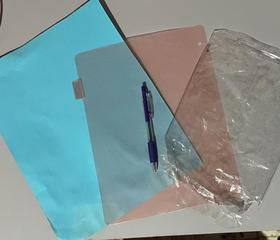
\includegraphics[scale=0.5]{Imagenes/Cuerpos_Luz_01.jpg}
\end{figure}
\end{frame}

\section{Leyes de la óptica geométrica}
\frame{\tableofcontents[currentsection, hideothersubsections]}
\subsection{Ley de reflexión}

\begin{frame}
\frametitle{Reflexión de la luz}
Cuando la luz llega a la superficie de un cuerpo, ésta se \textocolor{coolblack}{refleja total o parcialmente} en todas direcciones. 
\end{frame}
\begin{frame}
\frametitle{Reflexión de la luz}
Si la superficie es lisa como en un espejo, los rayos son reflejados o rechazados en una sola dirección y sentido.
\end{frame}
\begin{frame}
\frametitle{Reflexión superficie lisa}
\begin{figure}
    \centering
    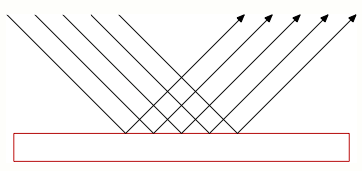
\includegraphics[scale=1]{Imagenes/Optica_Reflexion_001.png}
\end{figure}
\end{frame}
\begin{frame}
\frametitle{Reflexión superficie no lisa}
\begin{figure}
    \centering
    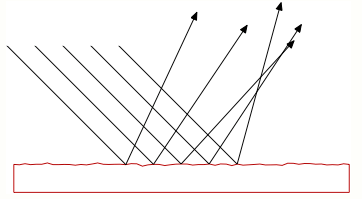
\includegraphics[scale=1]{Imagenes/Optica_Reflexion_002.png}
\end{figure}
\end{frame}
\begin{frame}
\frametitle{Nombrando a los rayos}
Al rayo de luz que llega al espejo se le nombra \textocolor{coquelicot}{incidente} y al rayo rechazado por él se le llama \textocolor{armygreen}{reflejado}.
\end{frame}
\begin{frame}
\frametitle{Leyes de reflexión}
Existen dos leyes de la reflexión propuestas por Descartes y son:
\pause
\setbeamercolor{item projected}{bg=aquamarine,fg=black}
\setbeamertemplate{enumerate items}{%
\usebeamercolor[bg]{item projected}%
\raisebox{1.5pt}{\colorbox{bg}{\color{fg}\footnotesize\insertenumlabel}}%
}
\begin{enumerate}[<+->]
\item El rayo incidente, la normal y el rayo reflejado se encuentran en un mismo plano.
\seti
\end{enumerate}
\end{frame}
\begin{frame}
\frametitle{Leyes de reflexión}
\setbeamercolor{item projected}{bg=aquamarine,fg=black}
\setbeamertemplate{enumerate items}{%
\usebeamercolor[bg]{item projected}%
\raisebox{1.5pt}{\colorbox{bg}{\color{fg}\footnotesize\insertenumlabel}}%
}
\begin{enumerate}[<+->]
\conti
\item El ángulo de reflexión es igual al ángulo de incidencia.
\end{enumerate}
\end{frame}
\begin{frame}
\frametitle{Leyes de la reflexión}
\begin{figure}
    \centering
    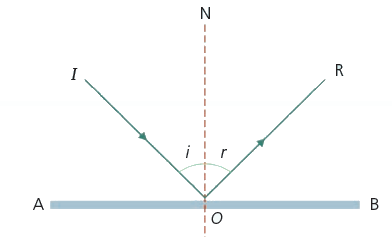
\includegraphics[scale=0.8]{Imagenes/Optica_Reflexion_01.png}
\end{figure}
\end{frame}

\subsection{Refracción de la luz}

\begin{frame}
\frametitle{La refracción de la luz}
La refracción de la luz consiste en la \textocolor{bulgarianrose}{desviación} que sufren los rayos luminosos cuando llegan a la superficie de separación entre \textocolor{burgundy}{dos sustancias o medios de diferente densidad}.
\end{frame}
\begin{frame}
\frametitle{La refracción de la luz}
Si éstos inciden perpendicularmente a la superficie de separación de las sustancias, no se refractan.
\end{frame}
\begin{frame}
\frametitle{La refracción de la luz}
La causa que origina la refracción de la luz es el \textocolor{bole}{cambio en la magnitud de la velocidad} de los rayos luminosos al penetrar a un medio de diferente densidad.
\end{frame}
\begin{frame}
\frametitle{La refracción de la luz}
Los rayos oblicuos que llegan a la superficie de separación entre dos medios se llaman \textocolor{lava}{incidentes} y los que se desvían al pasar por ésta se les nombra \textocolor{red}{refractados}.
\end{frame}
\begin{frame}
\frametitle{Refracción de la Luz}
\vspace*{-1cm}
\begin{figure}
    \centering
    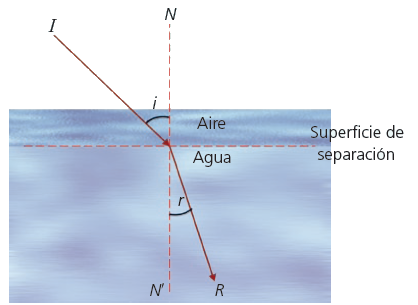
\includegraphics[scale=0.75]{Imagenes/Optica_Refraccion_01.png}
\end{figure}
\end{frame}

\subsection{Leyes de la refracción}

\begin{frame}
\frametitle{Las leyes de la refracción}
\setbeamercolor{item projected}{bg=americanrose,fg=white}
\setbeamertemplate{enumerate items}{%
\usebeamercolor[bg]{item projected}%
\raisebox{1.5pt}{\colorbox{bg}{\color{fg}\footnotesize\insertenumlabel}}%
}
\begin{enumerate}[<+->]
\item \textocolor{auburn}{Primera ley}: \pause el rayo incidente, la normal y el rayo refractado se encuentran siempre en el mismo plano.
\seti
\end{enumerate}
\end{frame}
\begin{frame}
\frametitle{Las leyes de la refracción}
\setbeamercolor{item projected}{bg=americanrose,fg=white}
\setbeamertemplate{enumerate items}{%
\usebeamercolor[bg]{item projected}%
\raisebox{1.5pt}{\colorbox{bg}{\color{fg}\footnotesize\insertenumlabel}}%
}
\begin{enumerate}[<+->]
\conti
\item \textocolor{blue-violet}{Segunda ley}: \pause para cada par de sustancias transparentes, la relación entre el seno del ángulo de incidencia y el seno del ángulo de refracción, \pause tiene un valor constante que recibe el nombre de \textocolor{ao}{índice de refracción} $n$.
\end{enumerate}
\end{frame}
\begin{frame}
\frametitle{Expresión para la refracción}
Matemáticamente esta ley se expresa:
\pause
\begin{align*}
n = \dfrac{\sin i}{\sin r}
\end{align*}
Donde:
\setbeamercolor{item projected}{bg=aureolin,fg=black}
\setbeamertemplate{enumerate items}{%
\usebeamercolor[bg]{item projected}%
\raisebox{1.5pt}{\colorbox{bg}{\color{fg}\footnotesize\insertenumlabel}}%
}
\begin{enumerate}[<+->]
\item $n$ es el índice de refracción (adimensional).
\item $i$ es el ángulo de incidencia.
\item $r$ es el ángulo de refracción.
\end{enumerate}
\end{frame}
\begin{frame}
\frametitle{La ley de Snell}
La segunda ley se conoce también como \textocolor{awesome}{ley de Snell}, \pause por ser el astrónomo y matemático holandés Willebrord Snell (1591-1626), quien la descubrió.
\end{frame}
\begin{frame}
\frametitle{La ley de Snell}
El índice de refracción también puede calcularse con el cociente de las \textocolor{carmine}{magnitudes de las velocidades} del primero y segundo medios, por lo que:
\pause
\begin{align*}
n = \dfrac{\sin i}{\sin r} = \dfrac{v_{1}}{v_{2}}
\end{align*}
\end{frame}
\begin{frame}
\frametitle{Índice de refracción}
La magnitud velocidad de la luz en el vacío es de \SI{3d5}{\kilo\meter\per\second}, \pause mientras que en el aire es de \SI{299030}{\kilo\meter\per\second} \pause y en el agua es de \SI{2.25d5}{\kilo\meter\per\second}.
\end{frame}
\begin{frame}
\frametitle{Índice de refracción}
La relación entre las magnitudes de las velocidades de la luz en el vacío y en un medio, \pause recibe el nombre de \textocolor{brown(web)}{índice de refracción del medio}.
\end{frame}
\begin{frame}
\frametitle{Valores del índice de refracción}
\begin{table}
\renewcommand{\arraystretch}{0.8}
\centering
\begin{tabular}{c | c}
Sustancia & Índice $n$\\ \hline
Aire & 1.003 \\ \hline
Agua & 1.33 \\ \hline
Alcohol & 1.36 \\ \hline
Vidrio & 1.5 \\ \hline
Diamante & 2.42 \\ \hline
\end{tabular}
\end{table}
\end{frame}
\begin{frame}
\frametitle{Enunciado del ejercicio}
Un rayo luminoso llega a la superficie de separación entre el aire y el vidrio, con un ángulo de incidencia de \ang{70}.
\\
\bigskip
\pause
Calcula el ángulo de refracción.
\end{frame}
\begin{frame}
\frametitle{Solución al ejercicio}
\textocolor{red}{Datos:}
\pause
\begin{eqnarray*}
\begin{aligned}
n_{\text{vidrio}} &= 1.5 \\[0.5em] \pause
\angle \, \text{inc} &= \ang{70} \\[0.5em] \pause
\angle \, \text{ref} &= \, ?
\end{aligned}
\end{eqnarray*}
\end{frame}
\begin{frame}
\frametitle{Resolviendo el ejercicio}
\textocolor{red}{Expresión:}
\pause
\begin{eqnarray*}
\begin{aligned}
n &= \dfrac{\sin i}{\sin r} \\[0.5em] \pause
\sin r &= \dfrac{\sin i}{n}
\end{aligned}
\end{eqnarray*}
\end{frame}
\begin{frame}
\frametitle{Resolviendo el ejercicio}
\textocolor{red}{Sustitución:}
\pause
\begin{eqnarray*}
\begin{aligned}
\sin r &= \dfrac{\sin \ang{70}}{1.5} = \pause \dfrac{0.93969}{1.5} = \\[0.5em] \pause
\sin r &= 0.6264
\end{aligned}
\end{eqnarray*}
Pero buscamos el valor del ángulo, por lo que aplicamos la función inversa: $\sin^{-1}$
\end{frame}
\begin{frame}
\frametitle{Resolviendo el ejercicio}
\begin{eqnarray*}
\begin{aligned}
\sin^{-1} (\sin r) &= \sin^{-1}(0.6264) = \\[0.5em] \pause
r &= \sin^{-1}(0.6264) = \\[0.5em] \pause
r &= \ang{38.789} = \\[0.5em] \pause
r &= \ang{38;47;21}
\end{aligned}
\end{eqnarray*}
\end{frame}
\begin{frame}
\frametitle{La ley de Snell}
Para un par dado de materiales, $a$ y $b$, la razón de los senos de los ángulos $\theta_{a}$ y $\theta_{b}$, donde los dos ángulos están medidos a partir de la normal a la superficie.
\end{frame}
\begin{frame}
\frametitle{La ley de Snell}
Es igual al inverso de la razón de los dos índices de refracción:
\pause
\begin{align*}
\dfrac{\sin \theta_{a}}{\sin \theta_{b}} = \dfrac{n_{b}}{n_{a}}
\end{align*}
\end{frame}
\begin{frame}
\frametitle{Enunciado del ejercicio}
En la siguiente figura el material $a$ es agua cuyo índice de refreacción es $1.33$ y el material $b$ es un vidrio con índice de refracción de $1.52.$
\end{frame}
\begin{frame}
\frametitle{Enunciado del ejercicio}
\begin{figure}
    \centering
    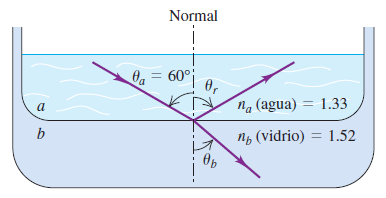
\includegraphics[scale=1]{Imagenes/Refraccion_Ondas_04.png}
\end{figure}
\end{frame}
\begin{frame}
\frametitle{Enunciado del ejercicio}
Si el rayo incidente forma un ángulo de \ang{60} con la normal, determina las direcciones de los rayos eflejado y refractado.
\end{frame}
\begin{frame}
\frametitle{Solución al ejercicio}
\textocolor{red}{Datos:}
\pause
\begin{eqnarray*}
\begin{aligned}
n_{\text{vidrio}} &= 1.52 \\[0.5em] \pause
n_{\text{agua}} &= 1.33 \\[0.5em] \pause
\angle \, \text{inc} &= \ang{60} \\[0.5em] \pause
\angle \, \text{reflejado} &= \, ?
\angle \, \text{refractado} &= \, ?
\end{aligned}
\end{eqnarray*}
\end{frame}
\begin{frame}
\frametitle{Resolviendo el ejercicio}
\textocolor{red}{Expresión:}
\pause
\begin{eqnarray*}
\begin{aligned}
\dfrac{\sin a}{\sin b} &= \dfrac{n_{b}}{n_{a}}  \\[0.5em] \pause
\sin b &= \dfrac{n_{a}}{n_{b}} \, \sin b \\[0.5em] \pause
\end{aligned}
\end{eqnarray*}
\end{frame}
\begin{frame}
\frametitle{El ángulo reflejado}
Por la ley de reflexión, el rayo reflejado forma un ángulo $\theta_{refl} = \ang{60}$ con respecto a la normal.
\end{frame}
\begin{frame}
\frametitle{Resolviendo el ejercicio}
\textocolor{red}{Sustitución:}
\pause
\begin{eqnarray*}
\begin{aligned}
\sin b &= \dfrac{1.33}{1.52} \, \sin \ang{60}  = \pause 0.758 = \\[0.5em] \pause
b &= \ang{49.3}
\end{aligned}
\end{eqnarray*}
\end{frame}
    

\section{Lentes}
\frame[allowframebreaks]{\tableofcontents[currentsection, hideothersubsections]}
\subsection{Tipos de lentes}

\begin{frame}
\frametitle{¿Qué es una lente?}
Las lentes son \textocolor{alizarin}{cuerpos transparentes} limitados por dos superficies esféricas o por una esférica y una plana.
\end{frame}
\begin{frame}
\frametitle{¿Para qué usar una lente?}
Las lentes se emplean a fin de desviar los rayos luminosos con base en las leyes de la refracción, para su estudio se dividen dos tipo:
\setbeamercolor{item projected}{bg=airforceblue,fg=black}
\setbeamertemplate{enumerate items}{%
\usebeamercolor[bg]{item projected}%
\raisebox{1.5pt}{\colorbox{bg}{\color{fg}\footnotesize\insertenumlabel}}%
}
\begin{enumerate}[<+->]
\item Convergentes.
\item Divergentes.
\end{enumerate}
\end{frame}

\subsection{Lentes convergentes}

\begin{frame}
\frametitle{Definición de lente convergente}
Las lentes convergentes son aquellas \textocolor{brightpink}{cuyo espesor va disminuyendo del centro hacia los bordes}, \pause razón por la cual su centro es más grueso que sus orillas.
\end{frame}
\begin{frame}
\frametitle{Propiedad de la lente convergente}
Tienen la propiedad de desviar los rayos hacia el eje y hacerlos converger en un punto llamado foco
\end{frame}
\begin{frame}
\frametitle{Lentes convergentes - Positivas}
\begin{figure}
    \centering
    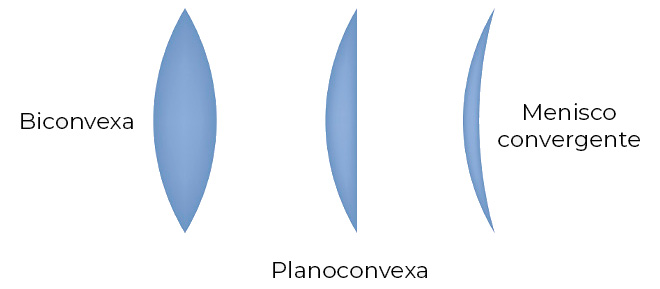
\includegraphics[scale=2]{Imagenes/Lentes_convergentes_01.jpg}
\end{figure}
\end{frame}
\begin{frame}
\frametitle{Símbolo de lente convergente}
\begin{figure}
    \centering
    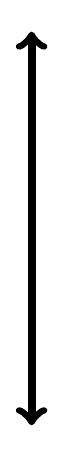
\begin{tikzpicture}
        \draw [<->, line width = 1mm] (0, -2.5) -- (0, 2.5);
    \end{tikzpicture}
\end{figure}
\end{frame}

\subsection{Lentes divergentes}

\begin{frame}
\frametitle{Definición de lente divergente}
En las lentes divergentes el \textocolor{cadmiumred}{espesor disminuye de los bordes hacia el centro}, \pause por lo que los extremos son más gruesos y desvían los rayos hacia el exterior, alejándolos del eje óptico de la lente.
\end{frame}
\begin{frame}
\frametitle{Lentes divergentes - Negativas}
\begin{figure}
    \centering
    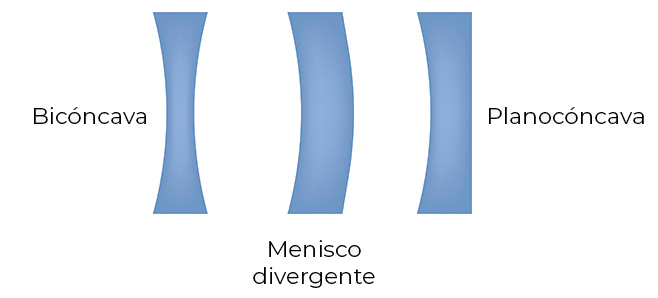
\includegraphics[scale=2]{Imagenes/Lentes_divergentes_01.jpg}
\end{figure}
\end{frame}
\begin{frame}
\frametitle{Símbolo de lente divergente}
\begin{figure}
    \centering
    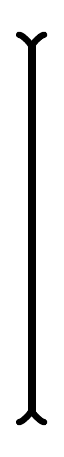
\begin{tikzpicture}
        \draw [>-<, line width = 1mm] (0, -2.5) -- (0, 2.5);
    \end{tikzpicture}
\end{figure}
\end{frame}

\subsection{Las partes de una lente}

\begin{frame}
\frametitle{Componentes de una lente}
Las principales partes de una lente son:
\pause
\setbeamercolor{item projected}{bg=aquamarine,fg=black}
\setbeamertemplate{enumerate items}{%
\usebeamercolor[bg]{item projected}%
\raisebox{1.5pt}{\colorbox{bg}{\color{fg}\footnotesize\insertenumlabel}}%
}
\begin{enumerate}[<+->]
\item El \textocolor{blush}{eje principal (E. P.)} , es la recta que pasa por el centro óptico y por los focos.
\item $L - L^{\prime}$ es el \textocolor{cardinal}{plano central de la lente} que es perpendicular al eje principal E.P.
\seti
\end{enumerate}
\end{frame}
\begin{frame}
\frametitle{Componentes de una lente}
\setbeamercolor{item projected}{bg=aquamarine,fg=black}
\setbeamertemplate{enumerate items}{%
\usebeamercolor[bg]{item projected}%
\raisebox{1.5pt}{\colorbox{bg}{\color{fg}\footnotesize\insertenumlabel}}%
}
\begin{enumerate}[<+->]
\conti
\item $C$ es el \textocolor{carnelian}{centro óptico de la lente}, cuando un rayo luminoso pasa por él no sufre ninguna desviación.
\item $F$ es el \textocolor{cobalt}{foco principal}, puntos donde se cruzan los rayos que llegan a la lente en forma paralela al eje principal.
\end{enumerate}
\end{frame}
\begin{frame}
\frametitle{Componentes de una lente}
El foco principal $F$ equivale a la \textocolor{cornellred}{distancia focal}, y es aquella distancia entre el centro óptico y el foco; \pause $2 \, F$ es la doble distancia focal.
\end{frame}
\begin{frame}
\frametitle{Componentes de una lente}
\begin{figure}
    \centering
    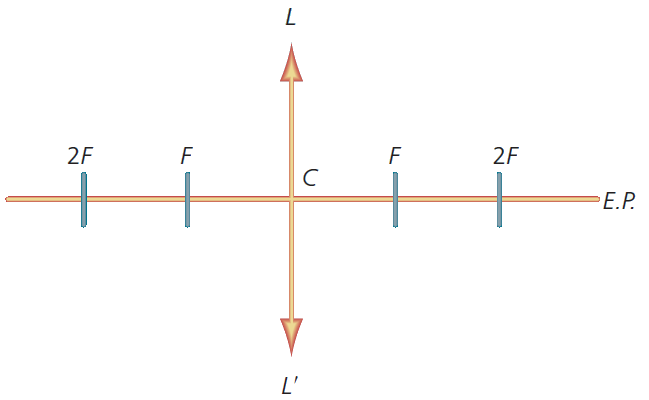
\includegraphics[scale=0.55]{Imagenes/Lentes_01.png}
\end{figure}
\end{frame}
\begin{frame}
\frametitle{Luz y lentes convergentes}
En las lentes convergentes, cualquier rayo luminoso que pase en forma paralela a su eje principal, al refractarse pasará por el foco principal.
\end{frame}
\begin{frame}
\frametitle{Luz y lentes convergentes}
\begin{figure}
    \centering
    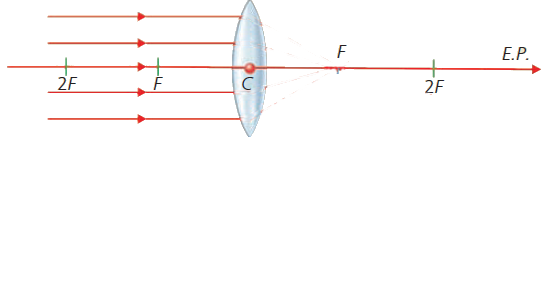
\includegraphics[scale=0.8]{Imagenes/Lentes_convergentes_02_02.png}
\end{figure}
\end{frame}
\begin{frame}
\frametitle{Luz y lentes convergentes}
\begin{figure}
    \centering
    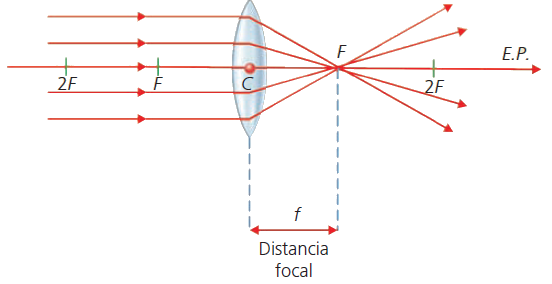
\includegraphics[scale=0.8]{Imagenes/Lentes_convergentes_02.png}
\end{figure}
\end{frame}
\begin{frame}
\frametitle{Luz y lentes divergentes}
En las lentes divergentes, el rayo que pase en forma paralela a su eje principal, al refractarse se separará como si procediera de un foco.
\end{frame}
\begin{frame}
\frametitle{Luz y lentes divergentes}
\begin{figure}
    \centering
    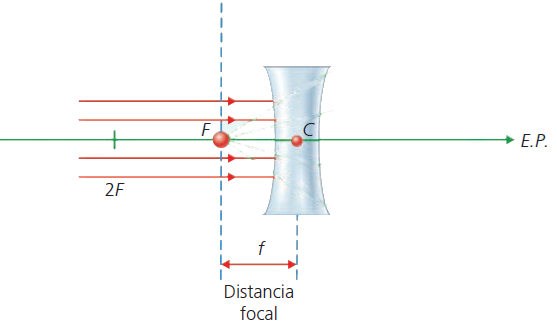
\includegraphics[scale=0.7]{Imagenes/Lentes_divergentes_02_02.png}
\end{figure}
\end{frame}
\begin{frame}
\frametitle{Luz y lentes divergentes}
\begin{figure}
    \centering
    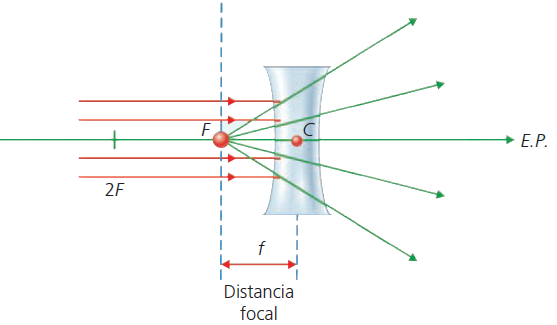
\includegraphics[scale=0.7]{Imagenes/Lentes_divergentes_02.png}
\end{figure}
\end{frame}

\subsection{Formación de imágenes}

\begin{frame}
\frametitle{Formación de imágenes}
\vspace*{-1cm}
El rayo 1 sale de un punto en el objeto y va paralelo al eje, luego se refracta a través del punto focal detrás.
\begin{figure}
    \centering
    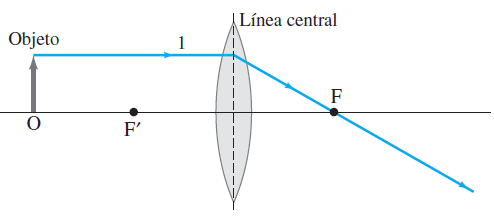
\includegraphics[scale=0.8]{Imagenes/Formacion_Imagen_01.png}
\end{figure}
\end{frame}
\begin{frame}
\frametitle{Formación de imágenes}
\vspace*{-1cm}
El rayo 2 pasa a través de $F^{\prime}$ enfrente de la lente; por consiguiente, es paralelo al eje detrás de la lente.
\begin{figure}
    \centering
    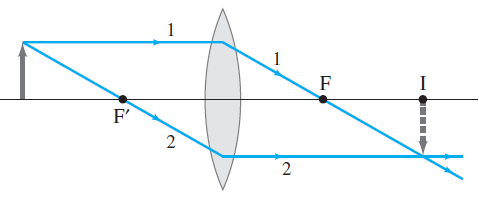
\includegraphics[scale=0.8]{Imagenes/Formacion_Imagen_02.png}
\end{figure}
\end{frame}
\begin{frame}
\frametitle{Formación de lentes}
\vspace*{-1cm}
El rayo 3 pasa recto a través del  centro de la lente (que se supone muy delgada).
\begin{figure}
    \centering
    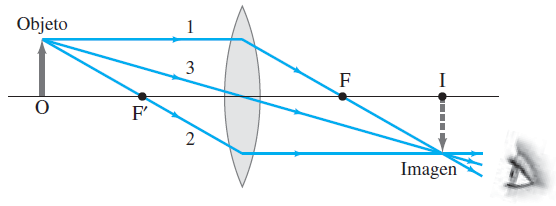
\includegraphics[scale=0.8]{Imagenes/Formacion_Imagen_03.png}
\end{figure}
\end{frame}
\begin{frame}
\frametitle{Tipo de imagen}
Dado que los rayos en realidad pasan a través de la imagen para el caso que hemos mostrado, \pause se trata de una \textocolor{bulgarianrose}{imagen real}.
\end{frame}
\begin{frame}
\frametitle{Formación en lente divergente}
\vspace*{-1cm}
El rayo 1 se dibuja paralelo al eje, pero no pasa a través del punto focal $F^{\prime}$ detrás de la lente.
\begin{figure}
    \centering
    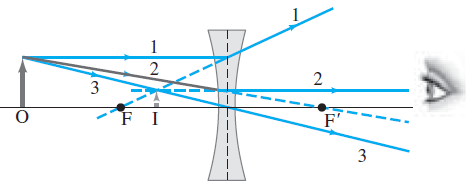
\includegraphics[scale=0.8]{Imagenes/Formacion_Imagen_04.png}
\end{figure}
\end{frame}
\begin{frame}
\frametitle{Formación en lente divergente}
En vez de ello, parece provenir desde el punto focal $F$ enfrente de la lente (línea punteada).
\end{frame}
\begin{frame}
\frametitle{Formación en lente divergente}
\vspace*{-1cm}
El rayo 2 se dirige hacia $F^{\prime}$ y la lente lo refracta paralelo al eje de la lente.
\begin{figure}
    \centering
    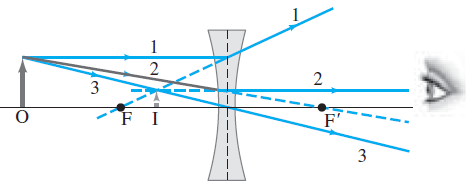
\includegraphics[scale=0.8]{Imagenes/Formacion_Imagen_04.png}
\end{figure}
\end{frame}
\begin{frame}
\frametitle{Formación en lente divergente}
\vspace*{-1cm}
El rayo 3 pasa directamente a través del centro de la lente.
\begin{figure}
    \centering
    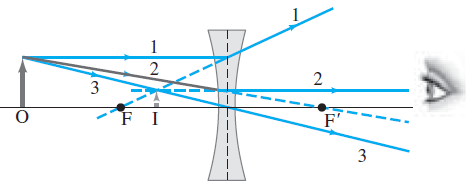
\includegraphics[scale=0.8]{Imagenes/Formacion_Imagen_04.png}
\end{figure}
\end{frame}

\begin{frame}
\frametitle{Formación en lente divergente}
\vspace*{-1cm}
Los tres rayos refractados parecen surgir de un punto a la izquierda de la lente. \pause
Éste es el punto de imagen, I.
\begin{figure}
    \centering
    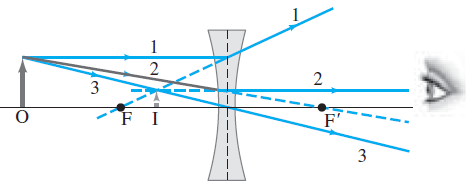
\includegraphics[scale=0.8]{Imagenes/Formacion_Imagen_04.png}
\end{figure}
\end{frame}
\begin{frame}
\frametitle{Tipo de imagen}
Puesto que los rayos no pasan a través de la imagen, \pause es una \textocolor{red}{imagen virtual}.
\end{frame}
\begin{frame}
\frametitle{Consideración importante}
Tomemos en cuenta de que el ojo no distingue entre imágenes reales y virtuales: ambas son visibles.
\end{frame}

\subsection{Ecuaciones lentes delgadas}

\begin{frame}
\frametitle{Elementos en la lente}
A continuación se presentan los elementos importantes tanto para una lente convergente como para una divergente, \pause que nos permitirán construir la llamada \textocolor{lava}{ecuación de una lente delgada}.
\end{frame}
\begin{frame}
\frametitle{Lente convergente}
\begin{figure}
    \centering
    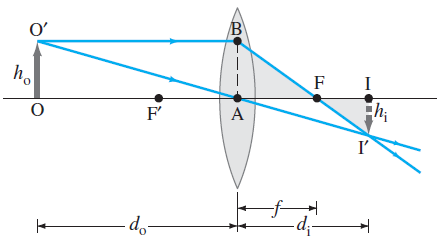
\includegraphics[scale=0.8]{Imagenes/Formacion_Imagen_05.png}
\end{figure}
\end{frame}
\begin{frame}
\frametitle{Ecuación de la lente convergente}
\begin{align*}
\dfrac{1}{f} = \dfrac{1}{d_{0}} + \dfrac{1}{d_{i}}
\end{align*}
A esta expresión se le llama \textocolor{cobalt}{ecuación de la lente delgada convergente}.
\end{frame}
\begin{frame}
\frametitle{Lente divergente}
\begin{figure}
    \centering
    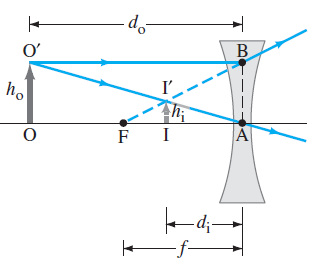
\includegraphics[scale=0.8]{Imagenes/Formacion_Imagen_06.png}
\end{figure}
\end{frame}
\begin{frame}
\frametitle{Ecuación de la lente divergente}
\begin{align*}
- \dfrac{1}{f} = \dfrac{1}{d_{0}} - \dfrac{1}{d_{i}}
\end{align*}
A esta expresión se le llama \textocolor{cobalt}{ecuación de la lente delgada divergente}.
\end{frame}
\begin{frame}
\frametitle{Convenciones de signos}
\setbeamercolor{item projected}{bg=aquamarine,fg=black}
\setbeamertemplate{enumerate items}{%
\usebeamercolor[bg]{item projected}%
\raisebox{1.5pt}{\colorbox{bg}{\color{fg}\footnotesize\insertenumlabel}}%
}
\begin{enumerate}[<+->]
\item La \textocolor{blue-violet}{distancia focal} es \textocolor{amethyst}{positiva para lentes convergentes} \pause y \textocolor{alizarin}{negativa para lentes divergentes}.
\seti
\end{enumerate}
\end{frame}
\begin{frame}
\frametitle{Convenciones de signos}
\setbeamercolor{item projected}{bg=aquamarine,fg=black}
\setbeamertemplate{enumerate items}{%
\usebeamercolor[bg]{item projected}%
\raisebox{1.5pt}{\colorbox{bg}{\color{fg}\footnotesize\insertenumlabel}}%
}
\begin{enumerate}[<+->]
\conti
\item La \textocolor{byzantium}{distancia del objeto es positiva} si el objeto está en el lado de la lente de donde proviene la luz; \pause de otro modo, \textocolor{bole}{es negativa}.
\seti
\end{enumerate}
\end{frame}
\begin{frame}
\frametitle{Convenciones de signos}
\setbeamercolor{item projected}{bg=aquamarine,fg=black}
\setbeamertemplate{enumerate items}{%
\usebeamercolor[bg]{item projected}%
\raisebox{1.5pt}{\colorbox{bg}{\color{fg}\footnotesize\insertenumlabel}}%
}
\begin{enumerate}[<+->]
\conti
\item La distancia de la imagen $d_{i}$ es positiva si la imagen está en el lado opuesto de la lente desde donde proviene la luz; si está en el mismo lado, $d_{i}$ es negativa.
\seti
\end{enumerate}
\end{frame}
\begin{frame}
\frametitle{Convenciones de signos}
De manera equivalente, la distancia de la imagen es positiva para una imagen real, y negativa para una imagen virtual.
\end{frame}
\begin{frame}
\frametitle{Convenciones de signos}
\setbeamercolor{item projected}{bg=aquamarine,fg=black}
\setbeamertemplate{enumerate items}{%
\usebeamercolor[bg]{item projected}%
\raisebox{1.5pt}{\colorbox{bg}{\color{fg}\footnotesize\insertenumlabel}}%
}
\begin{enumerate}[<+->]
\conti
\item La altura de la imagen, $h_{i}$, es positiva si la imagen está derecha, y negativa si la imagen está invertida en relación con el objeto.
\end{enumerate}
\end{frame}
\begin{frame}
\frametitle{Amplificación lateral}
La \textocolor{carmine}{amplificación lateral}, $m$, de una lente se define como la razón entre la altura de
la imagen y la altura del objeto:
\pause
\begin{align*}
m = \dfrac{h_{i}}{h_{0}} = - \dfrac{d_{i}}{d_{0}}
\end{align*}
\end{frame}
\begin{frame}
\frametitle{Amplificación lateral}
Para una \textocolor{coquelicot}{imagen derecha la amplificación es positiva}, \pause y para una \textocolor{awesome}{imagen invertida la amplificación es negativa}.
\end{frame}
\begin{frame}
\frametitle{Enunciado del ejercicio}
Un objeto de \SI{4}{\centi\meter} se coloca a \SI{20}{\centi\meter} de una lente convergente que tiene una distancia focal de \SI{12}{\centi\meter}.
\end{frame}
\begin{frame}
\frametitle{Enunciado del ejercicio}
Responde:
\setbeamercolor{item projected}{bg=bananayellow,fg=black}
\setbeamertemplate{enumerate items}{%
\usebeamercolor[bg]{item projected}%
\raisebox{1.5pt}{\colorbox{bg}{\color{fg}\footnotesize\insertenumlabel}}%
}
\begin{enumerate}[<+->]
\item ¿A qué distancia de la lente se forma la imagen?
\item ¿Cuál es su tamaño?
\end{enumerate}
\end{frame}
\begin{frame}
\frametitle{Resolviendo el ejercicio}
\vspace*{-0.5cm}
\textocolor{red}{Datos:}
\pause
\begin{align*}
h_{o} &= \SI{4}{\centi\meter} \\
h_{i} &= \, ? \\
f &= \SI{12}{\centi\meter} \\
d_{o} &= \SI{20}{\centi\meter} \\
d_{i} &= \, ?
\end{align*}
\end{frame}
\begin{frame}
\frametitle{Resolviendo el ejercicio}
\textocolor{red}{Expresiones:}
\pause
\begin{eqnarray*}
\begin{aligned}
&\text{a)} \quad \dfrac{1}{f} = \dfrac{1}{d_{o}} + \dfrac{1}{d_{i}} \pause \hspace{0.2cm} \Rightarrow \hspace*{0.2cm} \dfrac{1}{d_{i}} = \dfrac{1}{f} - \dfrac{1}{d_{o}} \\[0.5em] \pause
&\Rightarrow \hspace*{0.2cm} d_{i} = \dfrac{1}{\dfrac{1}{f} - \dfrac{1}{d_{0}}}
\end{aligned}
\end{eqnarray*}
\end{frame}
\begin{frame}
\frametitle{Resolviendo el ejercicio}
\textocolor{red}{Expresiones:}
\pause
\begin{eqnarray*}
\begin{aligned}
&\text{b)} \quad \dfrac{h_{i}}{h_{o}} = - \dfrac{d_{i}}{d_{o}} \pause \hspace{0.2cm} \Rightarrow \hspace*{0.2cm} h_{i} = - \dfrac{d_{i} \cdot h_{o}}{d_{o}} 
\end{aligned}
\end{eqnarray*}
\end{frame}
\begin{frame}
\frametitle{Resolviendo el ejercicio}
\textocolor{red}{Sustitución:}
\pause
\begin{eqnarray*}
\begin{aligned}
d_{i} = \dfrac{1}{\dfrac{1}{\SI{12}{\centi\meter}} - \dfrac{1}{\SI{20}{\centi\meter}}} = \pause \dfrac{1}{\dfrac{1}{\SI{30}{\centi\meter}}} = \pause \SI{30}{\centi\meter}
\end{aligned}
\end{eqnarray*}
\pause
\\[0.5em]
La imagen se forma a \SI{30}{\centi\meter} detrás de la lente.
\end{frame}
\begin{frame}
\frametitle{Resolviendo el ejercicio}
\textocolor{red}{Sustitución:}
\pause
\begin{eqnarray*}
\begin{aligned}
h_{i} &= - \dfrac{(\SI{30}{\centi\meter})(\SI{4}{\centi\meter})}{\SI{20}{\centi\meter}} = \\[0.5em] \pause
&= - \dfrac{\SI{120}{\square\centi\meter}}{\SI{20}{\centi\meter}} = \pause - \SI{6}{\centi\meter}
\end{aligned}
\end{eqnarray*}
\pause
\\[0.2em]
La imagen mide \SI{6}{\centi\meter} y está invertida con respecto al objeto.
\end{frame}
\begin{frame}
\frametitle{Enunciado del Ejercicio}
Un objeto se coloca a \SI{5}{\centi\meter} de una lente divergente que tiene una distancia focal de \SI{8}{\centi\meter}.
\\
\bigskip
\pause
¿A qué distancia se forma la imagen de la lente?
\end{frame}
\begin{frame}
\frametitle{Resolviendo el ejercicio}
\textocolor{red}{Datos:}
\pause
\begin{align*}
h_{o} &= \SI{5}{\centi\meter} \\
f &= \SI{8}{\centi\meter} \\
h_{i} &= \, ?
\end{align*}
\end{frame}
\begin{frame}
\frametitle{Resolviendo el ejercicio}
\textocolor{red}{Expresión:}
\pause
\begin{eqnarray*}
\begin{aligned}
- \dfrac{1}{f} &= \dfrac{1}{d_{0}} - \dfrac{1}{d_{i}} \\[0.5em] \pause
\dfrac{1}{d_{i}} &= \dfrac{1}{f} + \dfrac{1}{d_{0}} \\[0.5em] \pause
d_{i} &= \dfrac{1}{\dfrac{1}{f} + \dfrac{1}{d_{0}}} 
\end{aligned}
\end{eqnarray*}
\end{frame}
\begin{frame}
\frametitle{Resolviendo el ejercicio}
\textocolor{red}{Sustitución:}
\pause
\begin{eqnarray*}
\begin{aligned}
d_{i} &= \dfrac{1}{\dfrac{1}{\SI{8}{\centi\meter}} + \dfrac{1}{\SI{5}{\centi\meter}}} = \\[0.5em] \pause 
d_{i} &= \dfrac{1}{\dfrac{13}{40}} \\[0.5em] \pause 
d_{i} &= \dfrac{40}{13} = \pause \SI{3.076}{\centi\meter}
\end{aligned}
\end{eqnarray*}
\end{frame}
\begin{frame}
\frametitle{Enunciado del Ejercicio}
Cuál es:
\setbeamercolor{item projected}{bg=bananayellow,fg=ao}
\setbeamertemplate{enumerate items}{%
\usebeamercolor[bg]{item projected}%
\raisebox{1.5pt}{\colorbox{bg}{\color{fg}\footnotesize\insertenumlabel}}%
}
\begin{enumerate}[<+->]
\item la posición.
\item el tamaño de la imagen
\end{enumerate}
\pause
de una hoja de \SI{7.6}{\centi\meter} de alto colocada a \SI{1}{\meter} de la lente de una cámara con distancia focal de \SI{50.0}{\milli\meter}
\end{frame}
\begin{frame}
\frametitle{Resolviendo el ejercicio}
\vspace*{-1.5cm}
\textocolor{red}{Datos:}
\pause
\begin{align*}
h_{o} &= \SI{7.6}{\centi\meter} \\
d_{o} &= \SI{1}{\meter} \\
f &= \SI{50}{\milli\meter} \\
d_{i} &= \, ? \\
h_{i} &= \, ?
\end{align*}
\end{frame}
\begin{frame}
\frametitle{Resolviendo el ejercicio}
\vspace*{-1.5cm}
Para una lente negativa (divergente), la ecuación de la lente delgada es:
\\
\textocolor{red}{Expresión:}
\pause
\begin{eqnarray*}
\begin{aligned}
- \dfrac{1}{f} &= \dfrac{1}{d_{0}} - \dfrac{1}{d_{i}} \\[0.5em] \pause
\dfrac{1}{d_{i}} &= \dfrac{1}{f} + \dfrac{1}{d_{0}} \\[0.5em] \pause
d_{i} &= \dfrac{1}{\dfrac{1}{f} + \dfrac{1}{d_{0}}}     
\end{aligned}
\end{eqnarray*}
\end{frame}
\begin{frame}
\frametitle{Resolviendo el ejercicio}
\textocolor{red}{Sustitución:}
\pause
\begin{eqnarray*}
\begin{aligned}
d_{i} = \dfrac{1}{\dfrac{1}{\SI{5}{\centi\meter}} - \dfrac{1}{\SI{100}{\centi\meter}}} = \pause \dfrac{1}{\dfrac{19}{\SI{100}{\centi\meter}}} = \pause \SI{5.26}{\centi\meter}
\end{aligned}
\end{eqnarray*}
\end{frame}
\begin{frame}
\frametitle{Resolviendo el ejercicio}
La amplificación es:
\\
\textocolor{red}{Sustitución:}
\pause
\begin{eqnarray*}
\begin{aligned}
m &= - \dfrac{d_{i}}{d_{o}} = \pause - \dfrac{\SI{5.26}{\centi\meter}}{\SI{100}{\centi\meter}} = \\[0.5em] \pause
m &= - \num{0.0526}
\end{aligned}
\end{eqnarray*}
\end{frame}
\begin{frame}
\frametitle{Resolviendo el ejercicio}
De manera que:
\pause
\begin{eqnarray*}
\begin{aligned}
h_{i} &= m \, h_{o} = \pause (-0.0526)(\SI{7.6}{\centi\meter}) = \\[0.5em] \pause
h_{i} &= - \SI{0.40}{\centi\meter}
\end{aligned}
\end{eqnarray*}
\end{frame}
\begin{frame}
\frametitle{El resultado para $m$}
Revisa que el procedimiento para obtener la amplificación es el mismo que se ha ocupado, solo que se realizó un paso intermedio para obtener el valor de $m$.
\end{frame}
\begin{frame}
\frametitle{Resolviendo el ejercicio}
La distancia de la imagen $d_{i}$ resultó positiva, \pause así que la imagen está detrás de la lente.
\\
\bigskip
\pause
La altura de la imagen es $h_{i} = - \SI{0.40}{\centi\meter}$; \pause el signo menos significa que la imagen está invertida.
\end{frame}
\begin{frame}
\frametitle{Enunciado del ejercicio}
¿Dónde debe colocarse un pequeño insecto si una lente divergente con \SI{25}{\centi\meter} de distancia focal debe formar una imagen virtual a \SI{20}{\centi\meter} de la lente, en el mismo lado que el objeto?
\end{frame}
\begin{frame}
\frametitle{Resolviendo el ejercicio}
\vspace*{-1.5cm}
\textocolor{red}{Datos:}
\pause
\begin{align*}
f &= \SI{25}{\centi\meter}\\
d_{i} &= \SI{20}{\centi\meter} \\
d_{o} &= \, ?
\end{align*}
\end{frame}
\begin{frame}
\frametitle{Resolviendo el ejercicio}
\vspace*{-1.5cm}
Para una lente divergente (negativa), la distancia focal es negativa, \pause $f = - \SI{25}{\centi\meter}$:
\\
\textocolor{red}{Expresión:}
\pause
\begin{eqnarray*}
\begin{aligned}
- \dfrac{1}{f} &= \dfrac{1}{d_{0}} - \dfrac{1}{d_{i}} \\[0.5em] \pause
\dfrac{1}{d_{0}} &= - \dfrac{1}{f} + \dfrac{1}{d_{i}} \\[0.5em] \pause
d_{o} &= \dfrac{1}{- \dfrac{1}{f} + \dfrac{1}{d_{i}}}     
\end{aligned}
\end{eqnarray*}
\end{frame}
\begin{frame}
\frametitle{Resolviendo el ejercicio}
\vspace*{-1cm}
\textocolor{red}{Sustitución:}
\pause
\begin{eqnarray*}
\begin{aligned}
d_{o} &= \dfrac{1}{- \dfrac{1}{25} + \dfrac{1}{20}} = \pause \dfrac{1}{\dfrac{1}{\SI{100}{\centi\meter}}} = \\[0.5em] \pause
d_{o} &= \SI{100}{\centi\meter}     
\end{aligned}
\end{eqnarray*}
\pause
El objeto se debe de colocar a \SI{100}{\centi\meter} enfrente de la lente.
\end{frame}

\section{El ojo y la visión}
\frame{\tableofcontents[currentsection, hideothersubsections]}
\subsection{El ojo humano}

\begin{frame}
\frametitle{Anatomía del ojo humano}
\begin{figure}
    \centering
    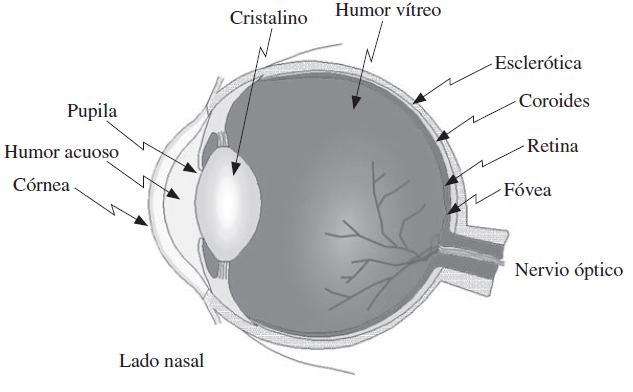
\includegraphics[scale=0.5]{Imagenes/Anatomia_Ojo_Humano.png}
\end{figure}
\end{frame}
\begin{frame}
\frametitle{Sobre la córnea}
La \textocolor{coquelicot}{córnea} es el primer elemento refractor del ojo \pause y contribuye con $43$ de las $58$ dioptrías que tiene el ojo.
\end{frame}
\begin{frame}
\frametitle{Sobre la córnea}
Su radio de curvatura es aproximadamente \SI{7.8}{\milli\meter} en la cara frontal, \pause \SI{6.5}{\milli\meter} en la cara posterior y un grueso de \SI{3.05}{\milli\meter}.
\end{frame}
\begin{frame}
\frametitle{Anomalías en la córnea}
Cualquier deformidad en la córnea da lugar al \textocolor{cerise}{error de refracción} que conocemos
con el nombre de \pause \textocolor{cerulean}{astigmatismo}.
\end{frame}
\begin{frame}
\frametitle{Anomalías en la córnea}
Una elongación del centro de la córnea recibe el nombre de \textocolor{red}{keratocono} \pause (kerato significa \enquote{córnea}).
\end{frame}
\begin{frame}
\frametitle{El cristalino}
El \textocolor{guppiegreen}{cristalino} es una lente flexible \pause cuya curvatura o poder de convergencia puede ser cambiada a voluntad para enfocar la imagen sobre la \textocolor{indigo(web)}{retina}.
\end{frame}
\begin{frame}
\frametitle{El cristalino}
A este proceso se le llama \textocolor{islamicgreen}{acomodación}.
\end{frame}
\begin{frame}
\frametitle{El ojo como transductor}
El ojo humano se asemeja a una cámara fotográfica.
\\
\bigskip
\pause
Tiene una \textocolor{burgundy}{lente} y \textocolor{byzantium}{una córnea curva}, \pause por lo que se forma una imagen real, disminuida e invertida.
\end{frame}
\begin{frame}
\frametitle{El ojo como transductor}
La imagen se forma en la \textocolor{bole}{retina}, la cual está constituida por células fotosensibles,
\end{frame}
\begin{frame}
\frametitle{El ojo como transductor}
La retina reacciona ante las distintas intensidades y colores de la luz que inciden sobre ella.
\end{frame}
\begin{frame}
\frametitle{El ojo como transductor}
Envía una proyección invertida de las cosas al cerebro, que se encarga de compensar esta inversión.
\end{frame}
\begin{frame}
\frametitle{El escotoma}
Observa en la siguiente figura el punto de la izquierda con el ojo derecho desde una distancia de alrededor de \SI{25}{\centi\meter}: \pause el pequeño cuadro desaparecerá.
\end{frame}
\begin{frame}
\frametitle{El escotoma}
\begin{figure}
    \centering
    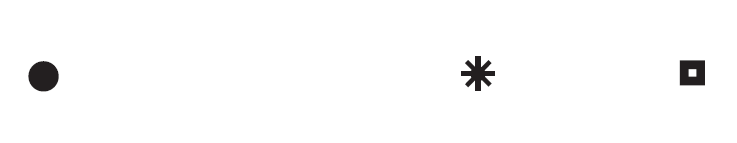
\includegraphics[scale=0.5]{Imagenes/Figura_Escotoma.png}
\end{figure}
\end{frame}
\begin{frame}
\frametitle{El escotoma}
Si la distancia se reduce a \SI{20}{\centi\meter}, la estrella desaparece en lugar del cuadro.
\end{frame}

\subsection{Anomalías en la visión}

\begin{frame}
\frametitle{Fallas en la visión}
Algunas personas padecen anomalías en su visión.
\end{frame}
\begin{frame}
\frametitle{La miopía}
El \textocolor{red}{ojo miope} no ve claramente los objetos lejanos ni los pequeños situados a distancias \enquote{visibles}
para un ojo sano.
\end{frame}
\begin{frame}
\frametitle{La miopía}
\begin{figure}
    \centering
    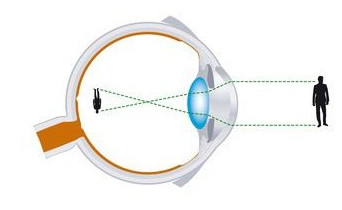
\includegraphics[scale=3.35]{Imagenes/Defectos_Vision_01_Miopia_01.jpg}
\end{figure}
\end{frame}
\begin{frame}
\frametitle{La miopía}
Las personas que padecen miopía tienen problemas para ver las letras con claridad y por ello tienen que acercar considerablemente la página a sus ojos.
\end{frame}
\begin{frame}
\frametitle{Corrigiendo la miopía}
Se corrige al usar cristales de bordes gruesos, es decir, lentes bicóncavas.
\end{frame}
\begin{frame}
\frametitle{La miopía}
\begin{figure}
    \centering
    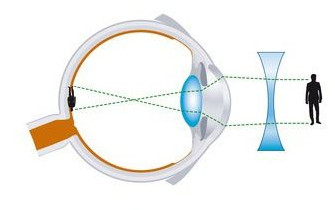
\includegraphics[scale=3.35]{Imagenes/Defectos_Vision_01_Miopia_02.jpg}
\end{figure}
\end{frame}    
\begin{frame}
\frametitle{La hipermetropía}
El \textocolor{ao}{ojo hipermétrope} no ve claramente los objetos cercanos, \pause porque la distancia mínima de visión
es mayor que la del ojo normal, por lo que se aleja el libro para leer.
\end{frame}
\begin{frame}
\frametitle{La hipermetropía}
Sin embargo, los objetos lejanos se ven claramente.
\end{frame}
\begin{frame}
\frametitle{La miopía}
\begin{figure}
    \centering
    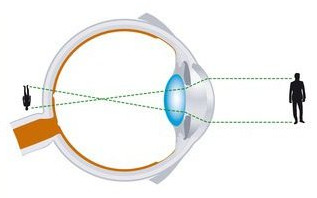
\includegraphics[scale=3.35]{Imagenes/Defectos_Vision_02_Hipermetropia_01.jpg}
\end{figure}
\end{frame}
\begin{frame}
\frametitle{Corrigiendo la hipermetropía}
Se corrige con cristales de bordes delgados, o sea, con lentes biconvexas.
\end{frame}
\begin{frame}
\frametitle{La miopía}
\begin{figure}
    \centering
    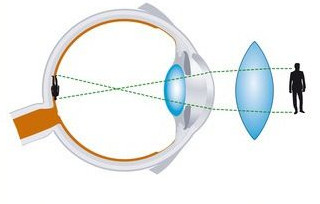
\includegraphics[scale=3.35]{Imagenes/Defectos_Vision_02_Hipermetropia_02.jpg}
\end{figure}
\end{frame}
\begin{frame}
\frametitle{La presbicia}
Hacia los 45 o 50 años, el ojo humano se vuele \textocolor{ao(english)}{présbita}: \pause suele ser un ojo \enquote{cansado} debido a
que la facultad de acomodación del cristalino ha disminuido.
\end{frame}
\begin{frame}
\frametitle{La presbicia}
El ojo présbita suele necesitar unas lentes para mirar de lejos y otras de cerca, \pause o bien, como es muy común, usar unas lentes bifocales.
\end{frame}
\begin{frame}
\frametitle{Diagrama de rayos - Ojo emétrope}
\begin{figure}
    \centering
    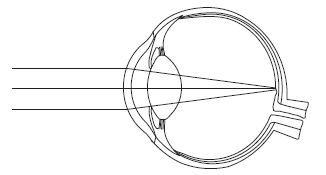
\includegraphics[scale=0.8]{Imagenes/Ojo_01_Emetrope.png}
\end{figure}
\end{frame}
\begin{frame}
\frametitle{Ojo miope}
\begin{figure}
    \centering
    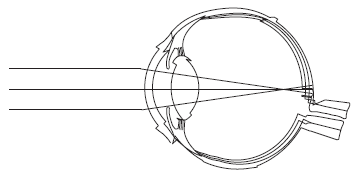
\includegraphics[scale=0.8]{Imagenes/Ojo_02_Miope.png}
\end{figure}
\end{frame}
\begin{frame}
\frametitle{Ojo hipermétrope}
\begin{figure}
    \centering
    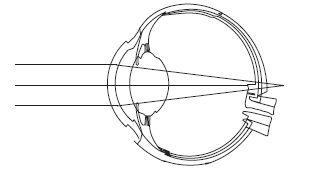
\includegraphics[scale=0.8]{Imagenes/Ojo_03_Hipermetrope.png}
\end{figure}
\end{frame}

\section{El color}
\frame{\tableofcontents[currentsection, hideothersubsections]}
\subsection{Definiciones}

\begin{frame}
\frametitle{¿Qué es el color?}
El color se debe a la propiedad que tienen todos los cuerpos de absorber y reflejar ciertas \textocolor{red}{radiaciones electromagnéticas}.
\end{frame}
\begin{frame}
\frametitle{¿Qué es el color?}
La mayoría de los colores que observamos de manera cotidiana, \pause son \textocolor{islamicgreen}{mezclas de longitudes de onda} que provienen de la absorción parcial de la luz blanca.
\end{frame}
\begin{frame}
\frametitle{¿Qué es el color?}
Casi todos los objetos deben su color a los filtros, pigmentos o pinturas, que absorben ciertas longitudes de onda de la luz blanca y reflejan las demás, \pause  estas longitudes de onda reflejadas son las que producen la sensación de color.
\end{frame}
\begin{frame}
\frametitle{¿Qué es el color?}
\begin{figure}
    \centering
    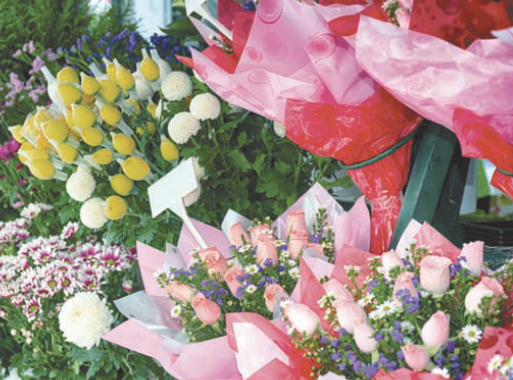
\includegraphics[scale=0.6]{Imagenes/Color_01.png}
\end{figure}
\end{frame}
\begin{frame}
\frametitle{¿Qué es el color?}
El mecanismo por el que las sustancias absorben la luz, depende de la estructura molecular de cada sustancia.
\end{frame}
\begin{frame}
\frametitle{La luz blanca}
La luz blanca del Sol es una mezcla de luces monocromáticas de longitudes de onda diferentes.
\end{frame}
\begin{frame}
\frametitle{La luz blanca}
Cuando una superficie recibe la luz solar y refleja todas las radiaciones de ésta, origina en la retina la sensación de color blanco.
\end{frame}
\begin{frame}
\frametitle{Reflejando colores}
Cuando una superficie absorbe todas las radiaciones, menos las azules, tiene un color azul; \pause cuando
sólo refleja las amarillas es de color amarillo.
\end{frame}
\begin{frame}
\frametitle{Reflejando colores}
\begin{figure}
    \centering
    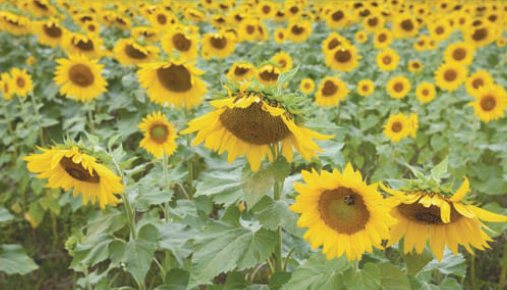
\includegraphics[scale=0.6]{Imagenes/Color_02.png}
\end{figure}
\end{frame}

\end{document}
